%%!TEX ROOT = ../mainCZ.tex




Vstupní data modelu jsou ve třech formátech: rastrovém, vektorovém a textovém. Do modelu vstupují informace o topografii řešeného území, informace o typech půd a vegetaci, informace o srážce atd. Základní formát vektorových dat je formát shapefile. Tento vektorový formát byl vytvořen firmou ESRI, ale je zpracovatelný i jinými GIS softwary. Parametry modelu jsou uloženy v atributové tabulce pod specifickým názvem pole. 
% Shapefile popisuje prvky jako body, linie nebo polygony. Každý prvek má obvykle nějaký atribut, který ho popisuje jako v tomto případě jméno, či typ půdy. 
V následujícím text jsou popsány náležitosti vstupních dat. 
% 
% Model pracuje s následujícími vstupy
Přehled vstupů do modelu je ukázán v tabulce~\ref{tab:vstupy}.
% 





% 

% 
\begin{sidewaystable}
% \begin{table}[]
\centering
\caption{Tabulka s přehledem vstulních dat modelu}
\label{tab:vstupy}
\small{
% \begin{tabular}{p{4cm}lp{2cm}p{5cm}}
\begin{tabular}{p{0.15\textwidth}lp{0.10\textwidth}p{0.25\textwidth}l}
\hline
Název                              & Typ dat                                               & Povinný / volitelný & Popis                                                                                      & Více v kapitole                                                 \\ \hline \hline
digitální model terénu             & \cellcolor[HTML]{96FFFB}{\color[HTML]{000000} raster} & Povinný           & Touto vrstvou se řídí i prostorová diskretizace                                                 & \ref{sec:vstupdmt}                                           \\ \hline
prostorové rozložení půd           & \cellcolor[HTML]{FFC702}vektor - polygony             & Povinný           & Atributová tabulka vrstvy identifikátor typu půdy                                               & \ref{sec:vstuppuda}                                          \\ \hline
prostorové rozložení typu vegetace & \cellcolor[HTML]{FFC702}vektor- polygony              & Povinný           & Atributová tabulka vrstvy identifikátor typu vegetace                                           & \ref{sec:vstupvegetace} a \ref{sec:upravatabulkyparametru}   \\ \hline
srážková data                      & .txt soubor                                           & Povinný           & Kumulativně zadaná srážka                                                                       & \ref{sec:vstupsrazka}                                        \\ \hline
maximální časový krok              & reálné číslo                                          & Povinný           & Model mění délku časového podle odtokových podmínek; doporučuje se 30 - 60 sekund               & \ref{sec:vstupkrok}                                          \\ \hline
výstupní adrešář                   & text                                                  & Povinný           & Adresář k uložení výsledků (při začátku výpočtu se adresář vyčistí!)                            & \ref{sec:vstupadresar}                                       \\ \hline
bodové výstupy hydrogramů          & \cellcolor[HTML]{FCFF2F}vektor - body                 & Volitelný         & Body, kde se vypíší výsledky.                                                                   & \ref{sec:vstupbody}                                          \\ \hline
typ výpočtu                        & text                                                  & Povinný           & Uživatel má na výběr: pouze plošní odtok, plošný i rýhový odtok, plošný rýhový odtok i odtok hydrografickou sítí               & \ref{sec:vstupryhovy}          \\ \hline
volba výcesměrného odtoku          & \cellcolor[HTML]{9698ED}logická proměnná              & Povinný           & Výchozí je jednosměrný odtok. Uživatel může zvolit vícesměnný odtok.                                                           & \ref{sec:vstupvicesmerny}      \\ \hline
paramtry půdy a vegetace           & \cellcolor[HTML]{67FD9A}tabulka                       & Povinný           & Tabulka parametrů půdy a vegetace. Názvy sloupců mají definované označení. Hodnoty se spojí s vektorovými vrstvami.            & \ref{sec:upravatabulkyparametru}\\ \hline
hydrografická síť                  & \cellcolor[HTML]{F8FF00}vektor - linie                & Volitelný         & Prostorové rozložení hydrografické sítě. Atributová tabulka obsahu identifikátor jednotlivých linií hydrografické sítě.        & \ref{sec:vodnitoky}             \\ \hline
parametry hydrografické sítě       & \cellcolor[HTML]{67FD9A}tabulka                       & Volitelný         & Tabulka parametrů jednotlivých úseků hydrografické sítě                                                                        &  \ref{sec:vodnitoky}     \\ \hline
volba arcgis výstupů               & \cellcolor[HTML]{9698ED}logická proměnná              & Povinný           & Výchozí formát výstupních rastrů je proprietární formát ERSI. Uživatel může zvolit textový formát ASCII.                       & --- \\ \hline
\end{tabular}
}
% \end{table}
\end{sidewaystable}
% \begin{itemize} \itemsep 0pt
% \item digitální model terénu
% \item shapefile půd
% \item shapefile využití území
% \item srážkový soubor
% \item časový krok výpočtu a celková doba simulace
% \item výstupní adresář
% \item bodová vrstva pro generování hydrogramů
% \item výstupní adresář
% \item typ výpočtu
% \item volba výcesměrného odtoku
% \item tabulka půd a vegetace a kód pro připojení
% \item shapefile hydrografické sítě
% \item tabulka vodních toků a kód pro připojení
% \item volitelné formy výstupů
% \end{itemize}


\pozn{
\textbf{Nutno dodělat}
\begin{itemize} \itemsep 0pt
\item upravit podle aktuálního stavu
\item upravit a zjednosušit tuto kapitolu
\item propojit s tabulkama co jsou jinde v textu
\item vložit sem tabulky parametrů výpočtu pokud nejsou jinde
\end{itemize}
}















\subsection{Digitální model terénu} \label{sec:vstupdmt} 

Rastr digitálního modelu terénu nebo také DMT, či anglicky DTM (Digital Terrain Model) je souvislý povrch území obvykle znázorňující morfologii určité části Země. DMT rastr je složen z jednotlivých buněk. Nejčastější formou jsou buňky čtvercové, ale mohou mít i jiný tvar. \pozn{smoderp dela jen ctverce, takze mozna zbytecna vedlejsi veta} Velikost buněk se liší v závislosti na velikosti zobrazovaného území. Pro účely modelu \smod by minimální velikost buněk měla být 2 metry, optimum je však 5 metrů a více. Důležitá je i celková rozloha rastru, tedy počet buněk. Model byl testován na rastrech o velikosti od několika málo tisíc buněk. DMT jednoho z testovacích, povodí Nučice, obsahuje přes 125 tisíc buněk. Příklad DMT dalšího testovacího povodí Býkovice je ukázán na obrázku~\ref{fig:bykovicedmt}.


\begin{figure}
  \centering
  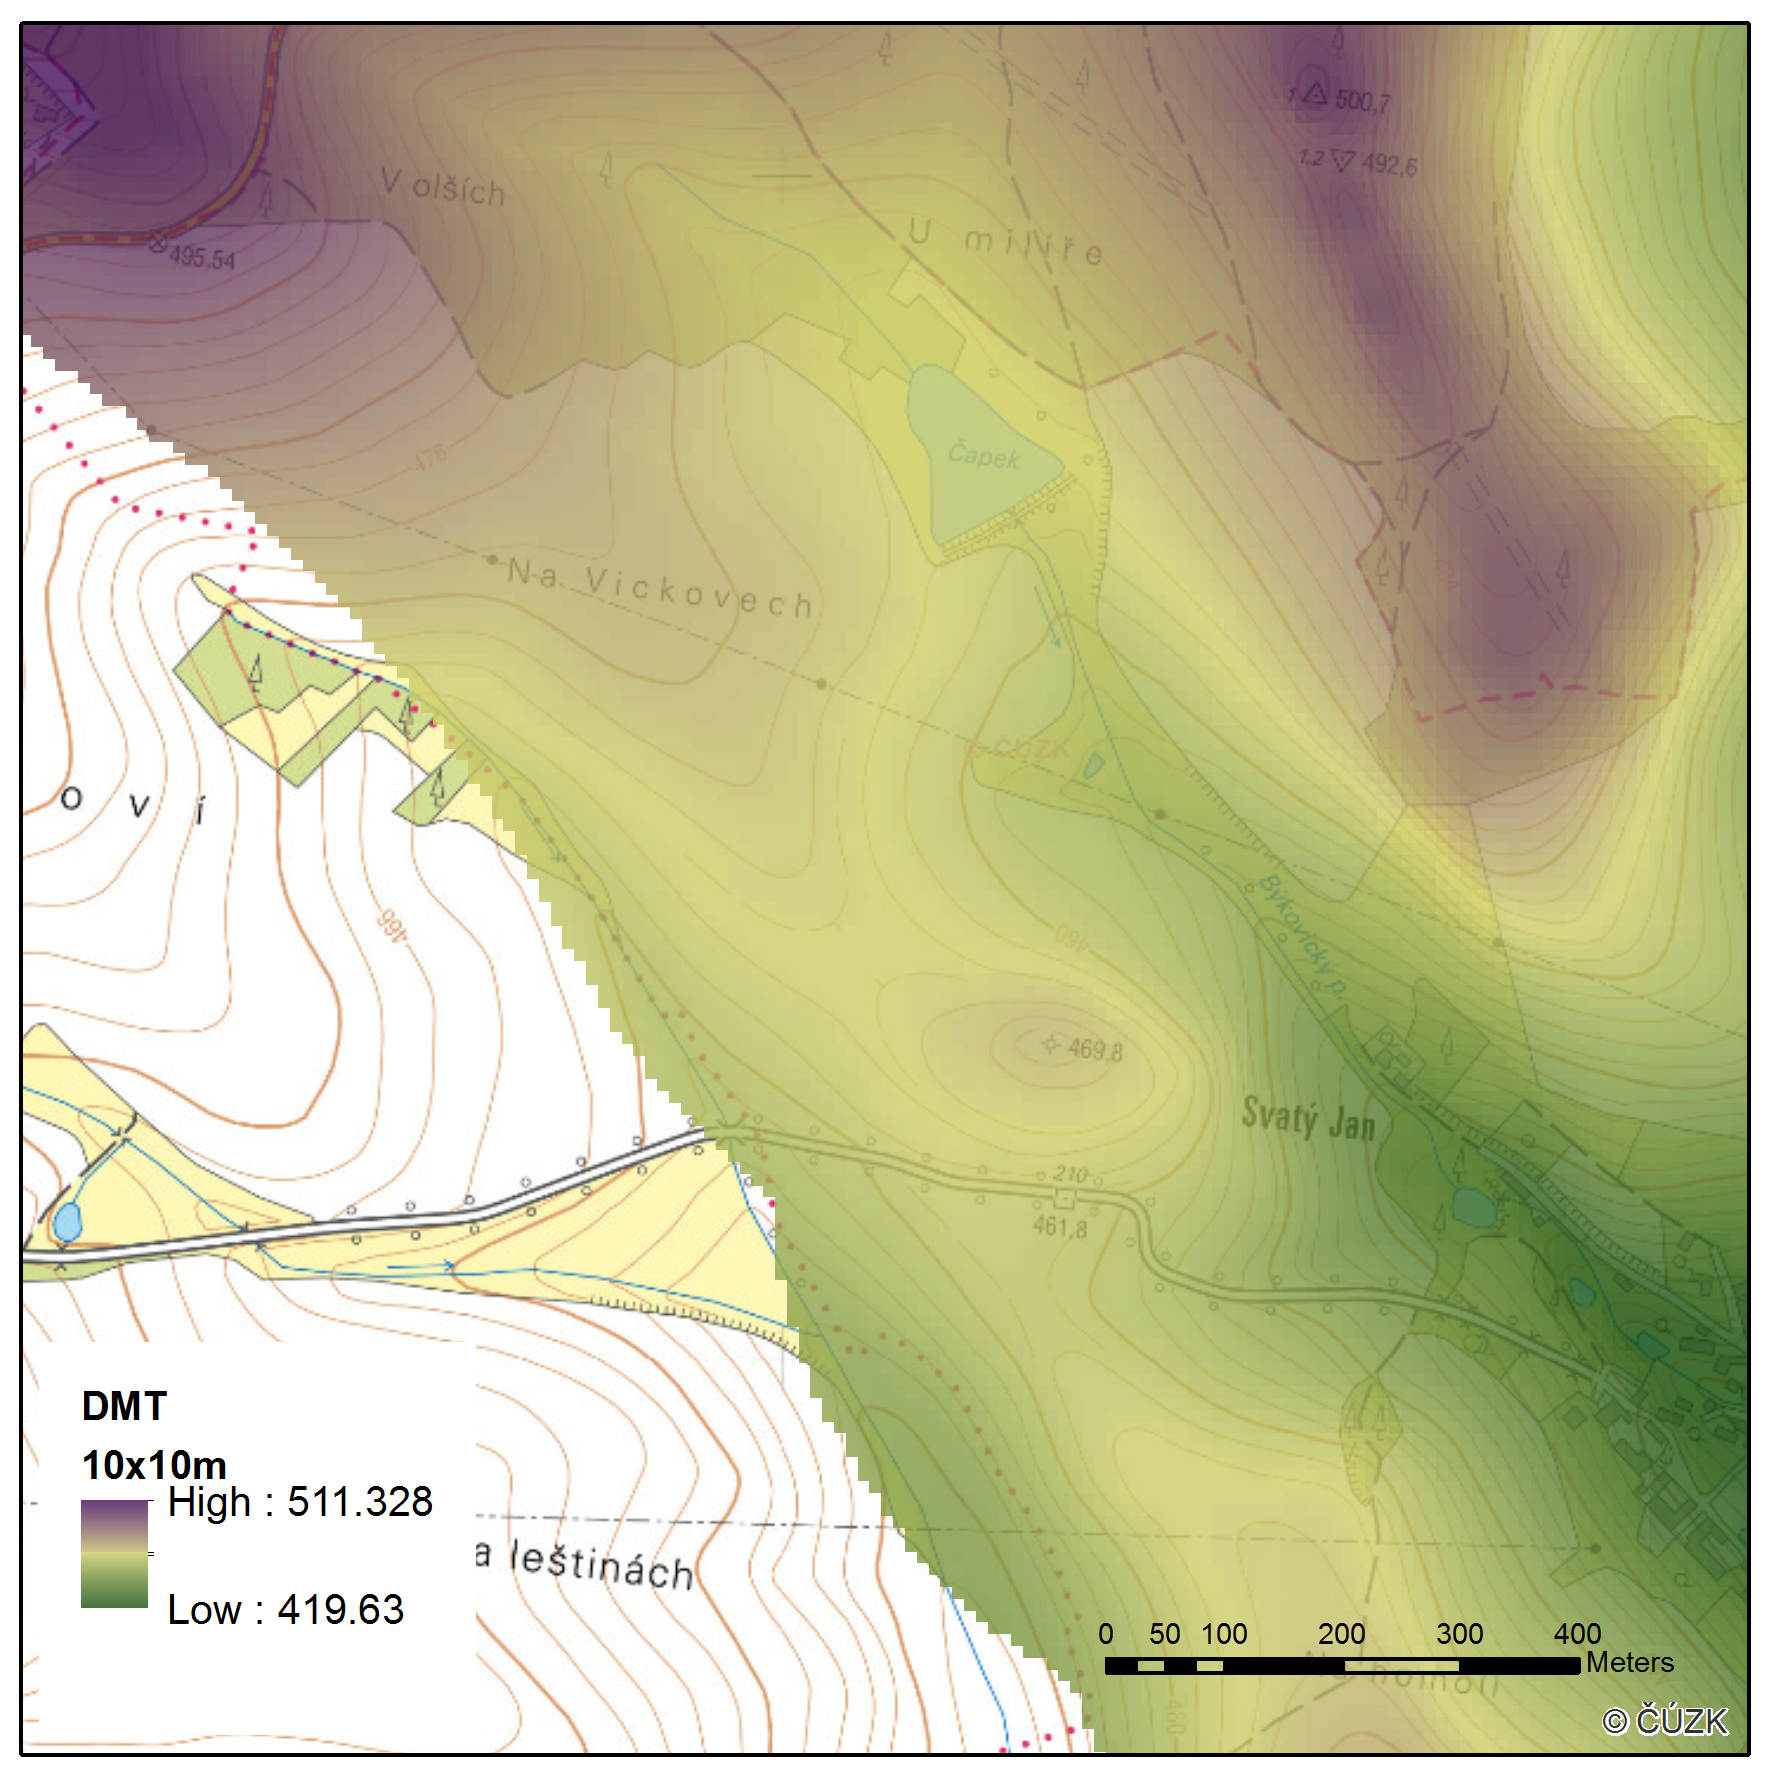
\includegraphics[width=0.5\textwidth]{./img/DMT_byk.png}
  \caption{Výřez digitálního modelu terénu povodí Býkovice}
  \label{fig:bykovicedmt}
\end{figure}

 
 
 
 
 
 
 
 
 
 
 
 
 
 
 
 
 
 
 
\subsection{Půdní data} \label{sec:vstuppuda}

Datové zdroje vlastností půd jsou v rámci České Republiky roztříštěné. Model \smod pracuje s jednou vstupní vrstvou půd. Příprava této vrstvy z dostupných dat je otázkou preprocessingu a spojení relevantních zdrojů. V zásadě jsou tři základní dostupné datové zdroje půdních vlastností. Odděleně připravená \pozn{to: jinou metodou pripravene si nejsem jist} data na zemědělské a lesní půdě nebo bezešvá vrstva půd KPP odpovídající měřítku 1:200000.

V České Republice se na zemědělské půdě standardně využívá rozdělení podle Novákovi klasifikace. Půda je rozdělena podle obsahu tzv. jílových částic na půdy \cite{kavka} \pozn{ v bib/bib.bib zadna polozka s oznacenim kavka neni...}:
\begin{itemize} \itemsep -3pt
  \item písčité
  \item hlinitopísčité
  \item písčitohlinité
  \item hlinité
  \item jílovitohlinité
  \item jílovité
  \item jíl
\end{itemize}

Na lesních půdách je v České Republice standardně využíván popis kategorií podle klasifikace USDA.
Obrázek~\ref{fig:pripravapar_vyrez}b ukazuje výřez připravené vrstvy. Pro určení charakteristik je nutné, aby atributová tabulka dané vrstvy obsahoval identifikátor půdního typu. Identifikátor odkazuje na půdní charakteristiky, které jsou ale uložené ve zvláštní tabulce (viz níže). Mezi půdní charakteristiky používané modelem patří: \acs{HyVod} - \acl{HyVod}; \acs{Sorb} - \acl{Sorb}; \acs{n} - \acl{n},  \acs{a} - \acl{a}, \acs{b} - \acl{b}, \acs{X} - \acl{X}, \acs{Y} - \acl{Y}. Hodnoty těchto parametrů jsou definované v tabulce, která popsána v kapitole~\ref{sec:upravatabulkyparametru}, v atributové tabulce je připraven pouze identifikátor daného polygonu. Fyzikální význam těchto parametrů a jejich implementace v modelu jsou popsány v části~\ref{cast:1} toho manuálu. 


% \begin{figure}
%   \centering
%   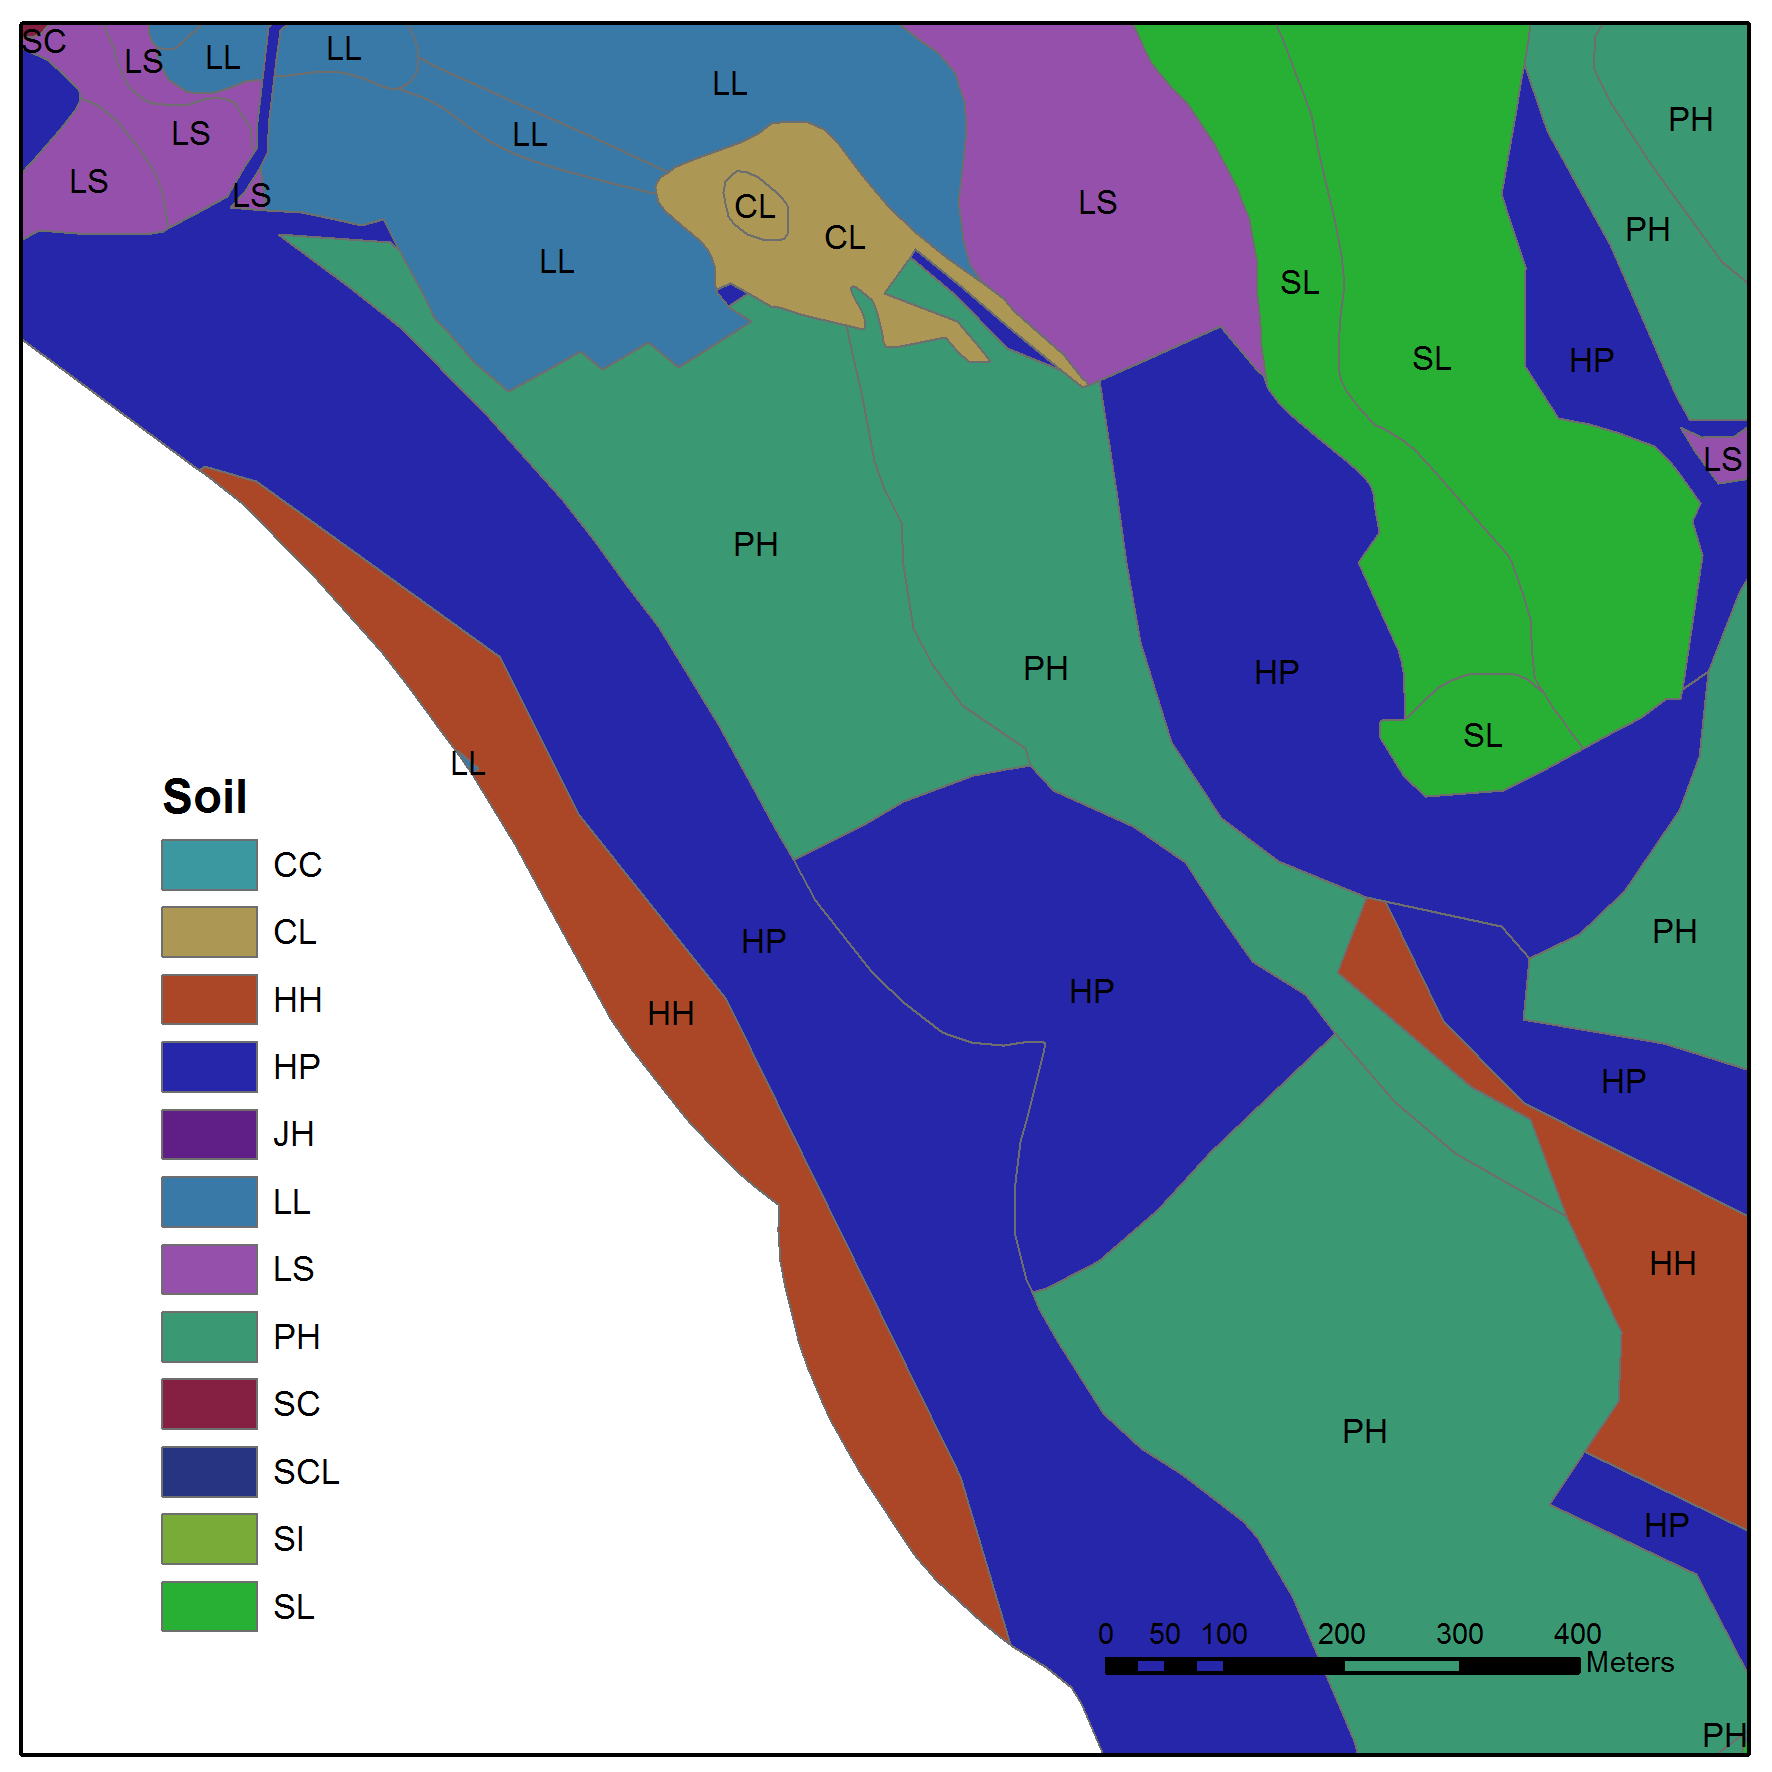
\includegraphics[width=0.5\textwidth]{./img/pudy.png}
%   \caption{výřez půdní mapy s vyznačenými půdními druhy}
%   \label{fig:bykovicepuda}
% \end{figure}
% 
%  
 
 
 
 
 
 
 
 
\subsection{Data o využití území} \label{sec:vstupvegetace}
\pozn{pk - doplnit zdroje takovych dat}
Obdobně jako u půdních dat je vstupem vektorový shapefile popisující využití území. Mezi základní typy pro které byl model testován patří:
\begin{itemize} \itemsep -3pt
  \item atropogení a zpevněné plochy  
  \item holá půda bez vegetace
  \item les
  \item sad
  \item travní porosty
  \item zemědělské plodiny širokořádkové\footnote{Širokořádkové plodiny jsou například brambory, kukuřice, řepa, sója a slunečnice.}
  \item zemědělské plodiny úzkořádkové\footnote{Úzkořádkové plodiny jsou obiloviny nebo řepka.}
\end{itemize}


Shapefile popisující využití území je na obrázku~\ref{fig:pripravapar_vyrez}c. Obdobně jako u půd v předchozí sekci je třeba atributovou tabulku tohoto shapefilu doplnit o identifikátor daného využití území. Tento identifikátor odkazuje na charakteristiky daného povrchu definované v dalším vstupech (popsáno v sekci~\ref{sec:upravatabulkyparametru}). Parametry, související s využitím území, které vstupující do modelu jsou zejména \acs{PotI} - \acl{PotI} a \acs{Lai} - \acl{Lai}. Jejich konkrétní použití je popsáno v části~\ref{cast:1} toho manuálu. 
% 
% \begin{figure}
%   \centering
%   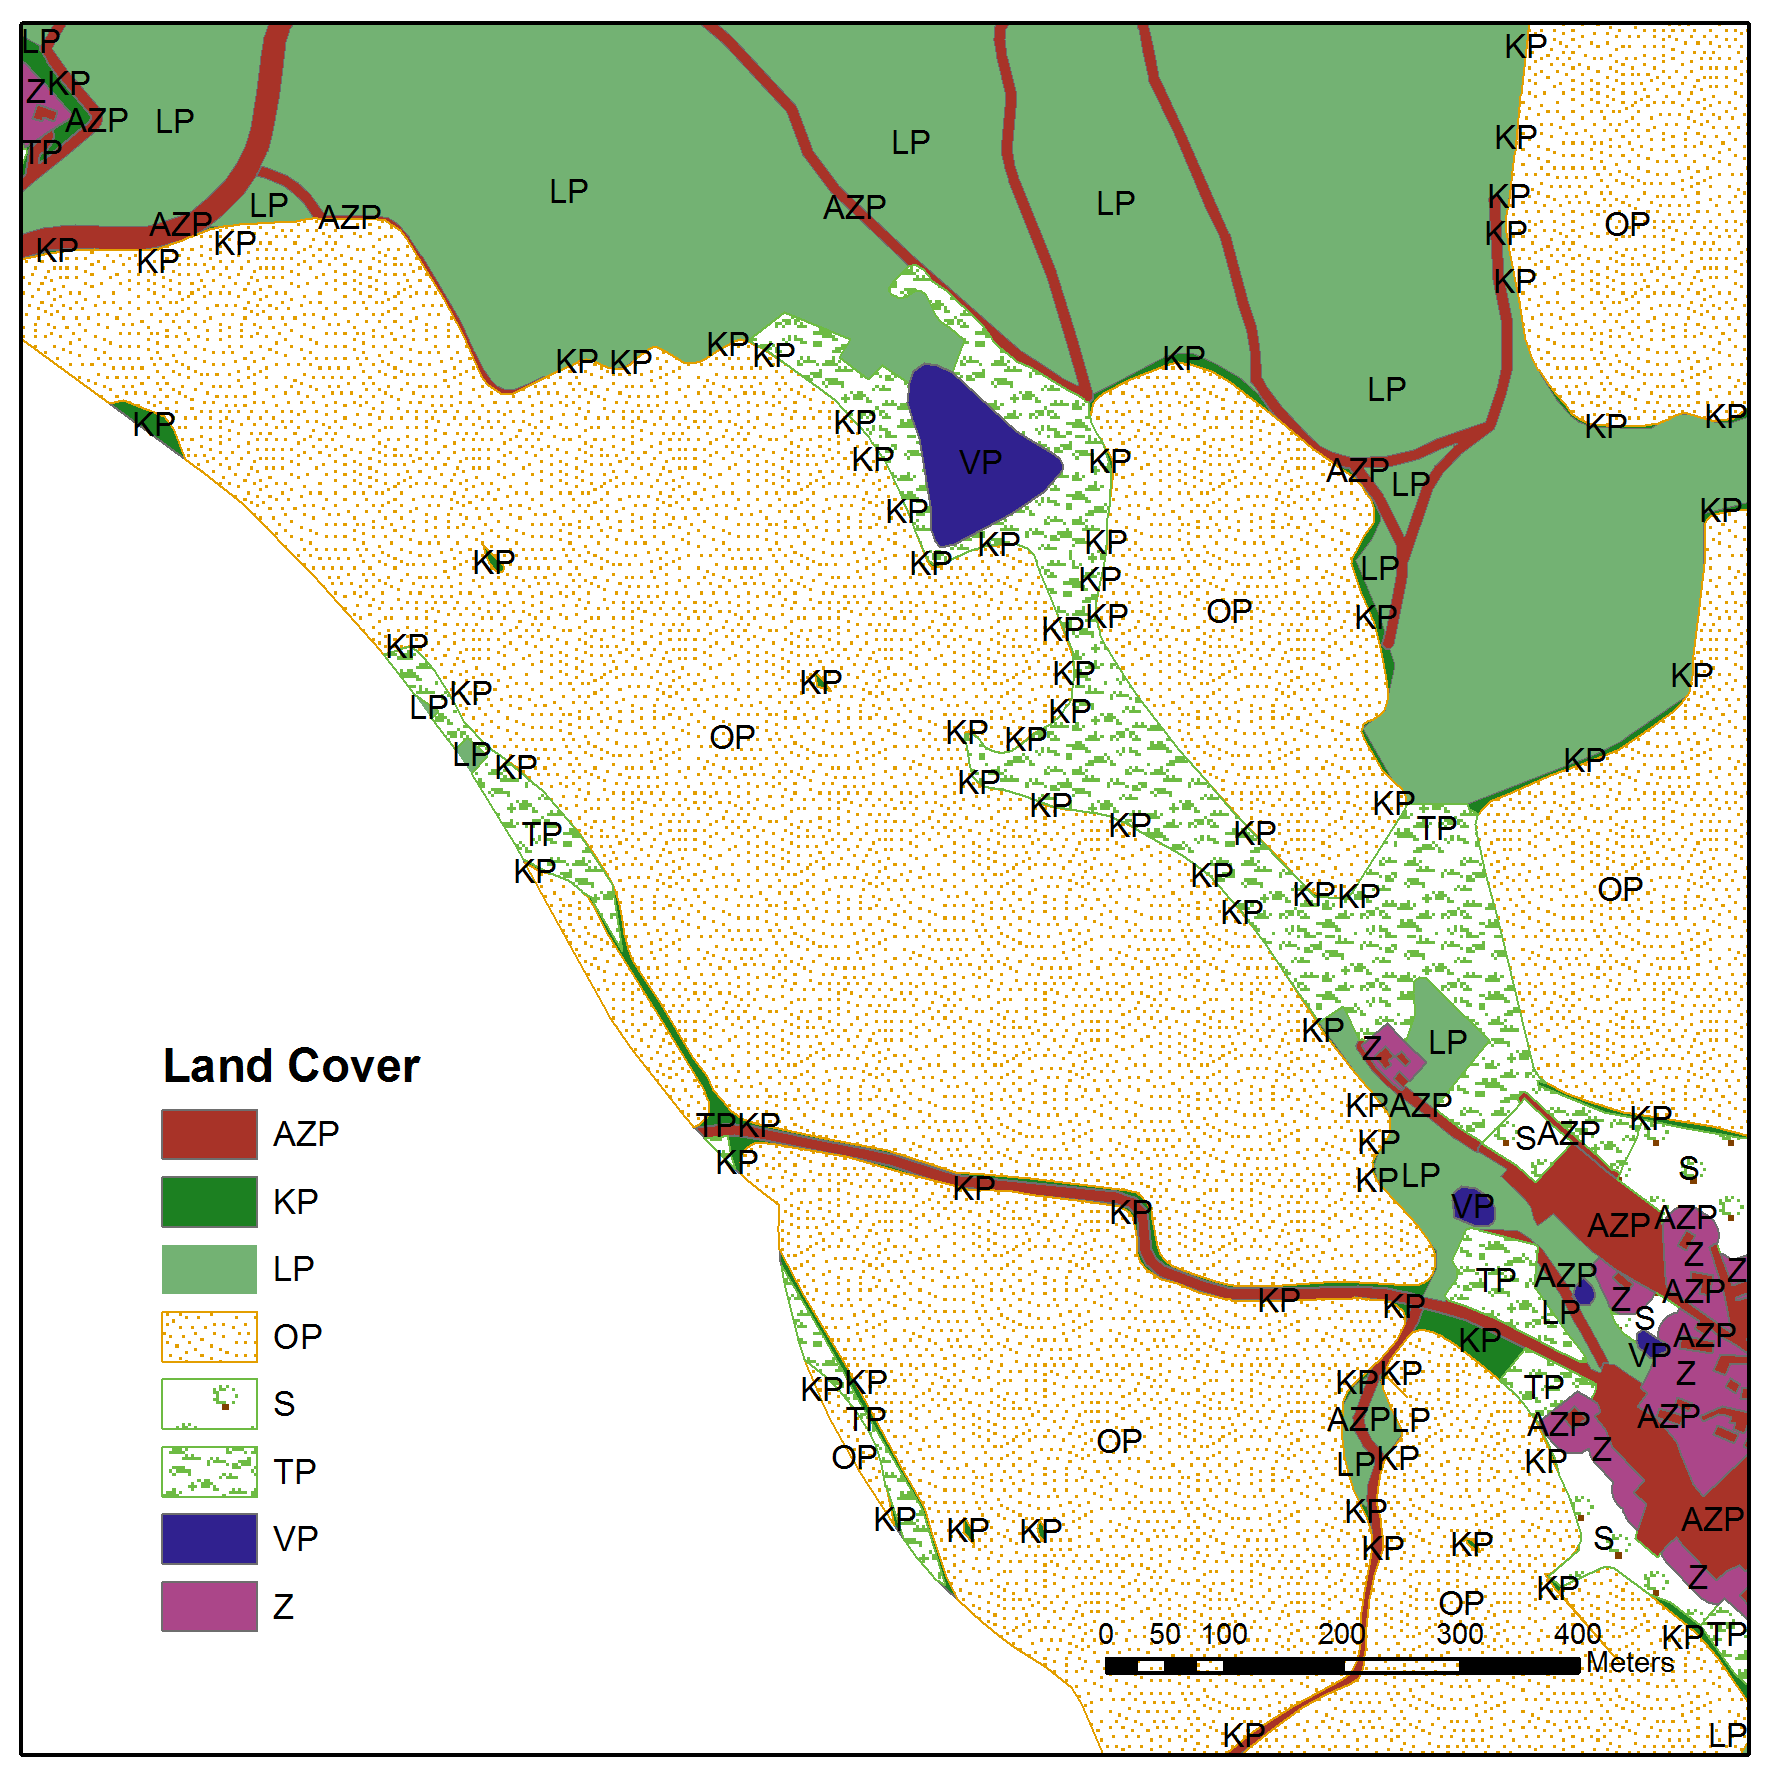
\includegraphics[width=0.5\textwidth]{./img/LandCover.png}
%   \caption{Ukázka vektorové vrstvy využití území -  Land Cover}
%   \label{fig:bykovicevegetace}
% \end{figure}
% 
% 
% 







\subsection{Tabulka parametrů půdy a využití území}  \label{sec:upravatabulkyparametru}

Tento vstup je tabulka, která obsahuje hodnoty jednotlivých parametrů popsaných v předešlých kapitolách a části~\ref{cast:1} toho manuálu. Na tuto tabulku se odkazují identifikátory půdního typu a typu využití území v atributových tabulkách polygonových vrstev. Tato tabulka může být do modelu vlože jako textový soubor. Na obrázku~\ref{fig:pripravapar_vyrez}e je ukázán příklad takové tabulky. V prvních dvou sloupcích jsou identifikátory (id) typu půd (Soil) a typu využití území (Land Co.). Spojením těchto dvou id jsou označeny parametry pro danou kombinaci typu půdy a využití území (třetí sloupec v tabulce na obrázku~\ref{fig:pripravapar_vyrez}e s označením soilveg). Význam jednotlivých veličin je popsán v tabulce~\ref{tab:soilveg}. Při přípravě dat je nutné dodržet označení parametrů!

Na obrázku~\ref{fig:pripravapar_vyrez} jsou i ukázky jednotlivých vektorových vrstev před (obrázek~\ref{fig:pripravapar_vyrez}b a ~\ref{fig:pripravapar_vyrez}c) a po protnutí (intersect; obrázek~\ref{fig:pripravapar_vyrez}d). 

% Na prvním řádku je ukázka odpovídající id půdního typu z obrázku~\ref{fig:bykovicepuda} HP a id typu využití území z obrázku~\ref{fig:bykovicevegetace} TP, které jsou v tabulce na obrázku~\ref{fig:tabsoilveg} spojeny na HPTP. Tímto způsobem je program schopen propojit prostorové uspořádání pud a typu vegetace s příslušnými charakteristikami. Spojení identifikátorů z atributových tabulkách polygonových vrstev prování program automaticky. Uživatel musí pouze zaručit aby se identifikátory v nastavené v atributových tabulkách polygonových vrstev schodovali s identifikátory v tabulce půdních charakteristik a charakteristik vegetace. Princip přípravy a propojení rozložení typů a vegetačního pokryvu s odpovídajícími parametry je naznačen na obrátku~\ref{}
% 
% Hlavničky druhého až posledního sloupce jsou povinné. Jejich význam je popsán v tabulce~\ref{tab:soilve g}. Názvy v druhém až posledním sloupečku musí být zadány malými písmeny.
% \begin{figure}
%   \centering
%   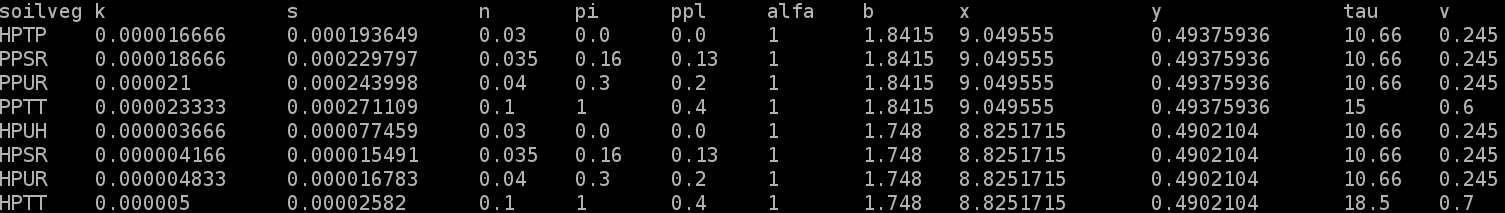
\includegraphics[width=1.0\textwidth]{./img/tabsoilveg.png}
%   \caption{Ukázka tabulky s charakteristikami půd a vegetace. Význam veličin v jednotlivých sloupcích je popsán v tabulce~\ref{tab:soilveg}.}
%   \label{fig:tabsoilveg}
% \end{figure}


% \begin{figure}
%   \centering
%   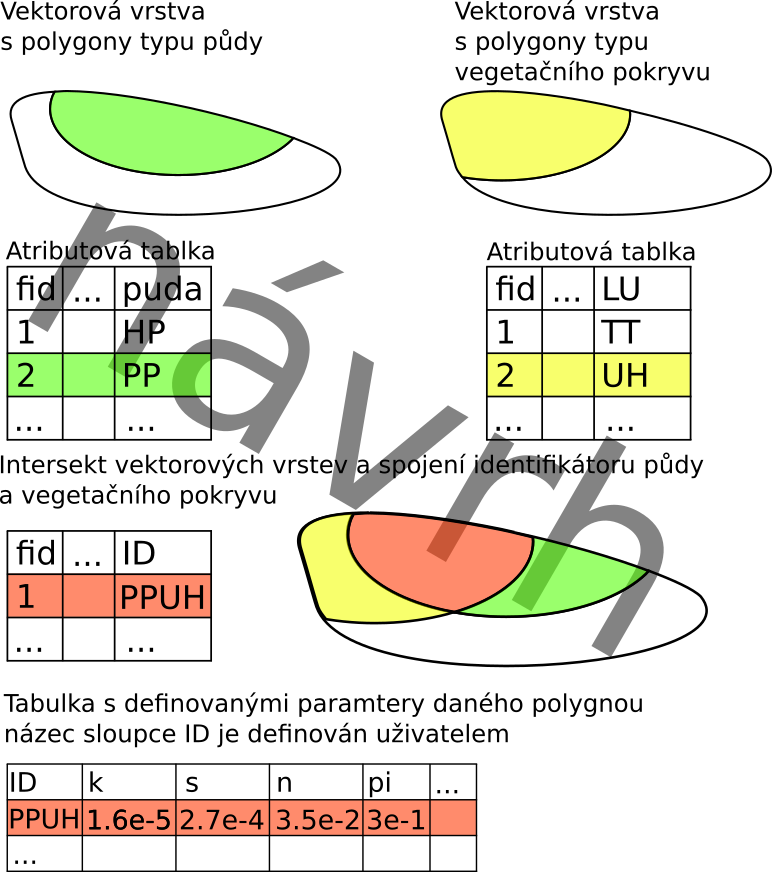
\includegraphics[width=0.75\textwidth]{./img/spojenistabulkou.png}
%   \caption{Princip propojení atributových tabulek vektorových vrstev s tabulkou obsahující jednotlivé parametry}
%   \label{fig:pripravapar_detail}
% \end{figure}



\begin{figure}[h!]
  \centering
%   \includegraphics[width=0.9\textwidth]{./img/kTabulce_soilveg.png}
  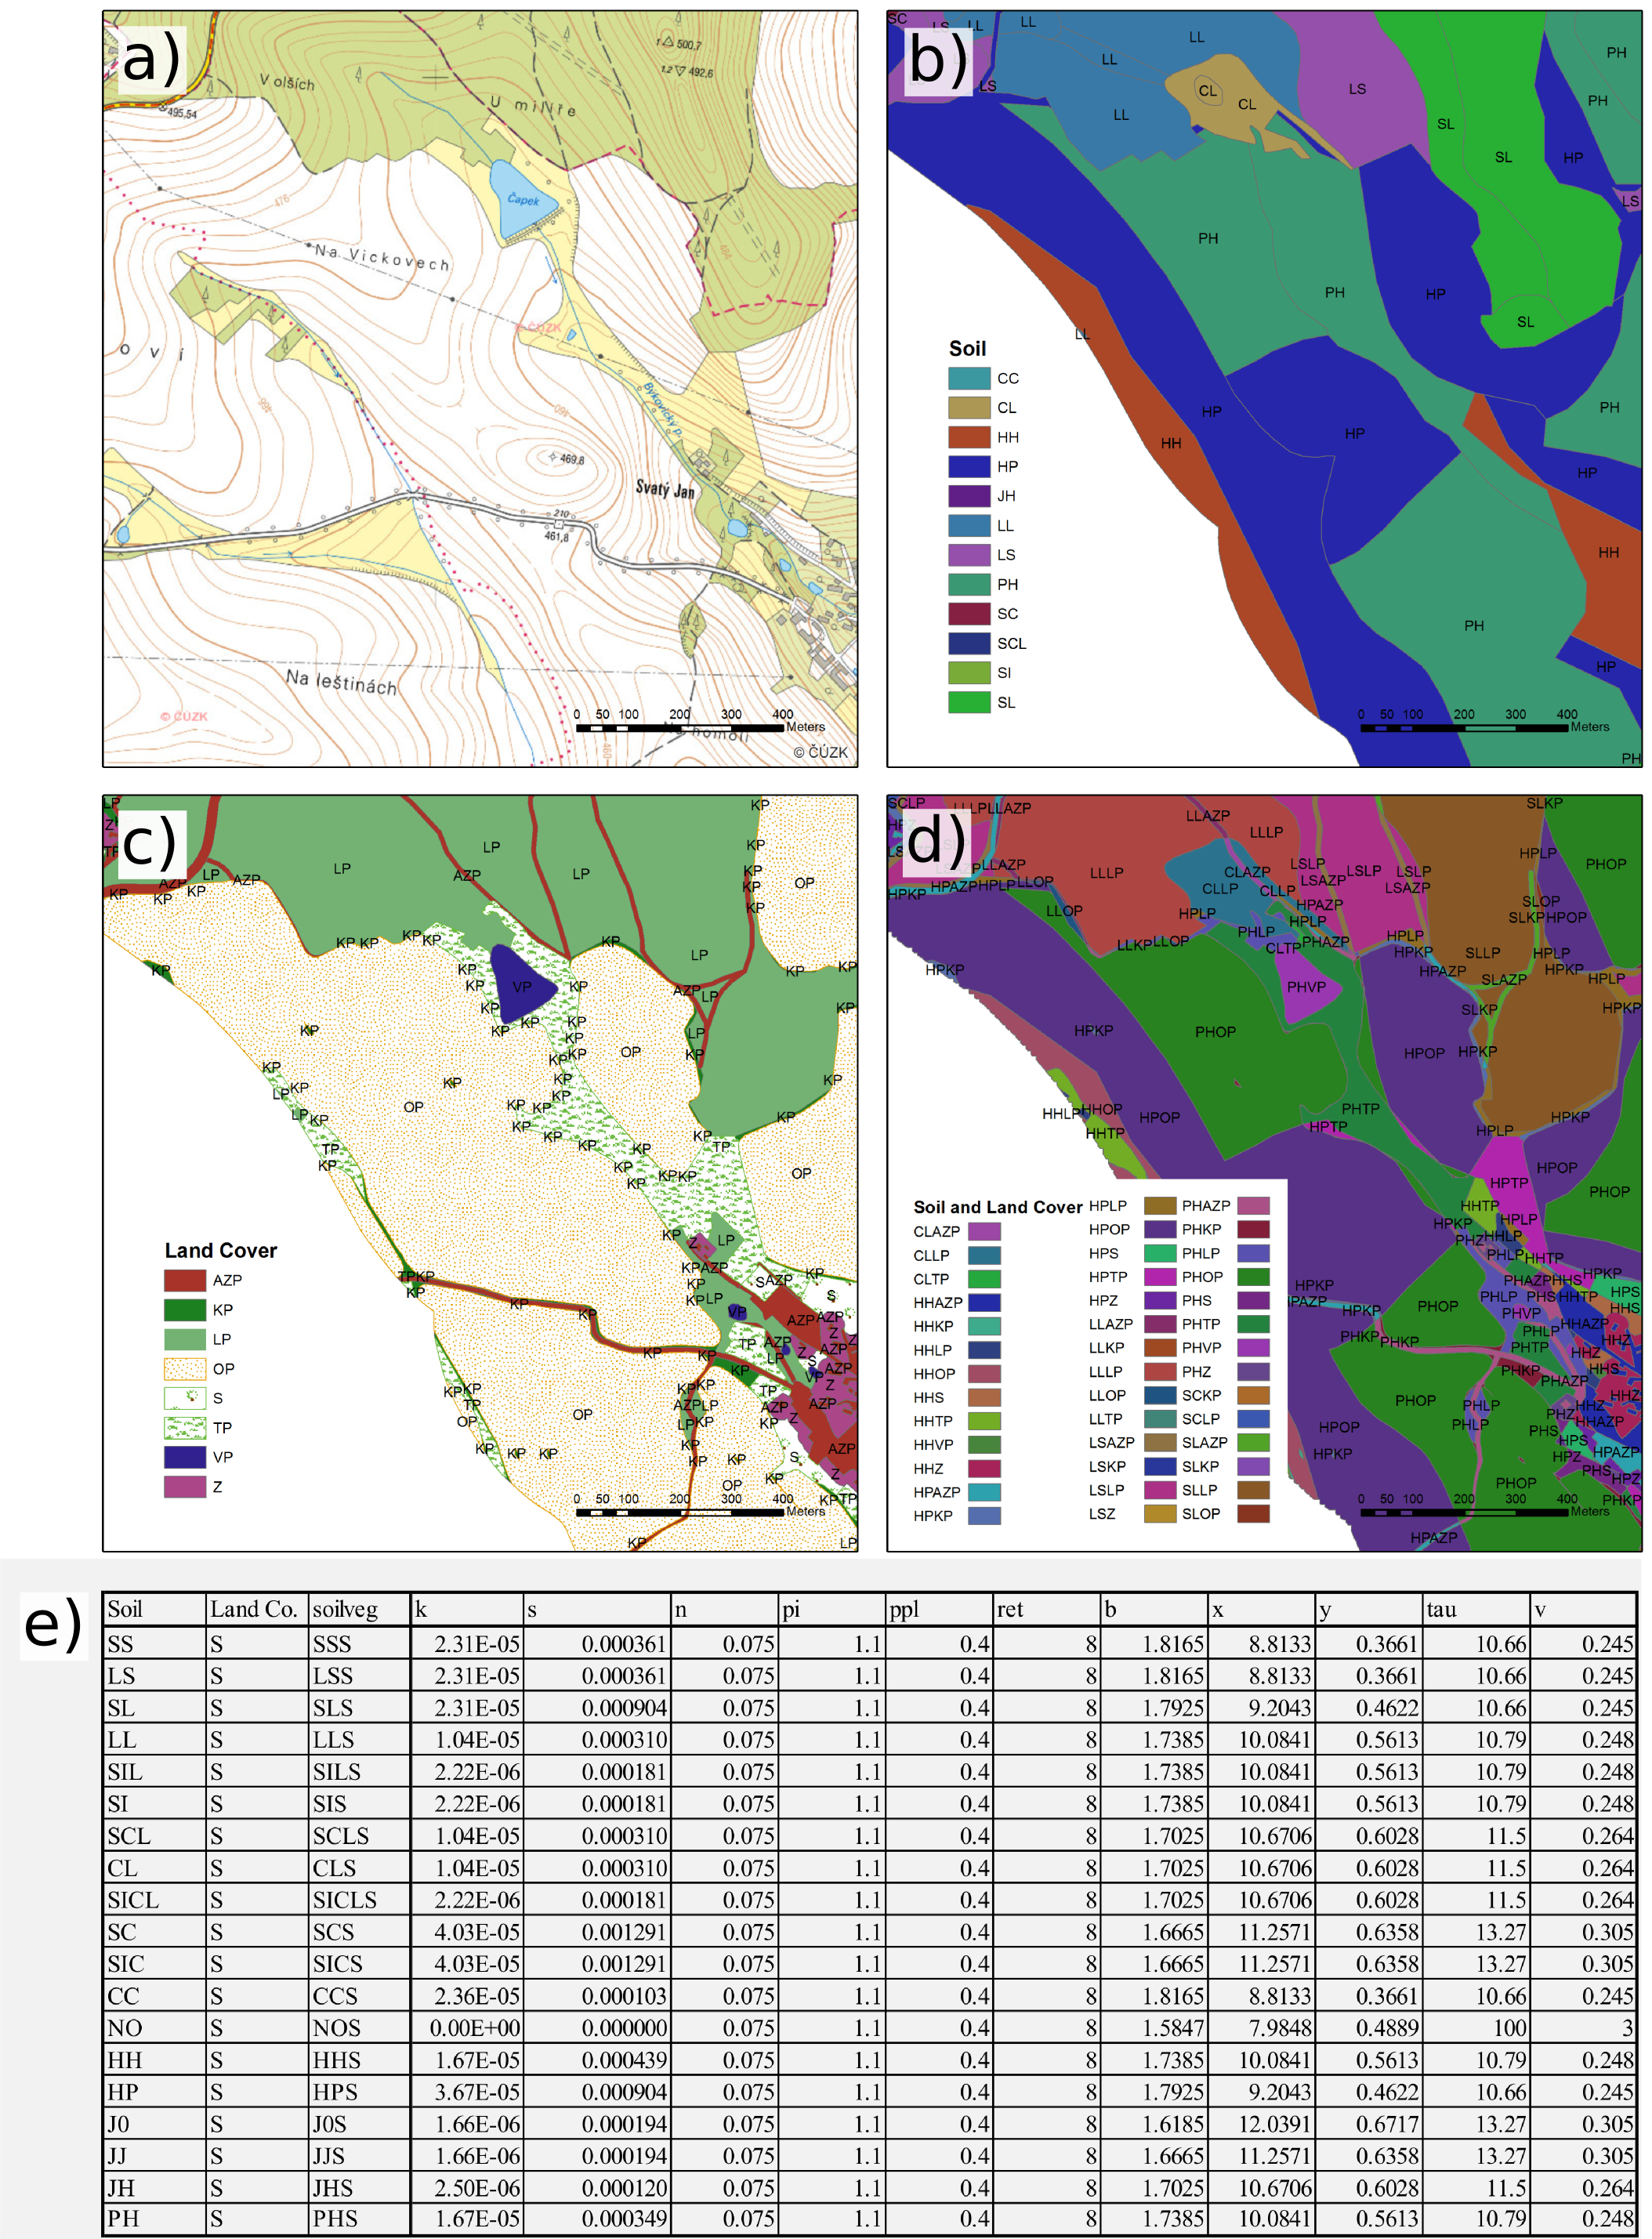
\includegraphics[width=0.9\textwidth]{./img/LUplusTAB.png} 
  \caption{Princip propojení vektorových vrstev s tabulkou obsahující parametry typu půd a vegetace. a): mapa daného území;  b): rozložení typu půdy; c):  rozložení typu vegetačního pokryvu; d): protnutí obou předchozích vrstev; e): tabulka s parametry}
  \label{fig:pripravapar_vyrez}
\end{figure}

\begin{table}%[!htp]
  \centering
  \caption{Přehled parametrů charakterizujících půdní typ a typ vegetačního pokryvu}
  {\small
    \begin{tabular}{p{1.5cm}lp{4cm}}
    \hline
    Hlavička v tabulce & Symbol & Popis \\
    \hline \hline
    k&\acs{HyVod}  & \acl{HyVod} \\
    s&\acs{Sorb}   & \acl{Sorb} \\
    n&\acs{n}      & \acl{n}\\
    pi&\acs{PotI}   & \acl{PotI}\\
    ppl&\acs{Lai}    & \acl{Lai} \\
    ret&\acs{ret}    & \acl{ret} \\
    b&\acs{b}      & \acl{b} \\
    x&\acs{X}      & \acl{X} \\
    y&\acs{Y}      & \acl{Y} \\
    tau&\acs{taucrit}& \acl{taucrit} \\
    v&\acs{vcrit}  & \acl{vcrit} \\
    \hline
    \end{tabular}%
  }
  \label{tab:soilveg}%
\end{table}%




\pozn{\textbf{nebo co toto} ty obrázky mám i zvlášť, @@@jj dal bych je zvlášť, dá se napsat popisek ke každému zvlášť i jeden společný (obr 5a, 5b, 5c....)}


\pozn{ Meze jednotlivých parametrů jsou podrobněji popsány v kapitole XXX. 
Součástí manuálu jsou i vzorové tabulky (do prilohy).}



\subsection{Srážkový soubor} \label{sec:vstupsrazka}

Dalším vstupem je soubor obsahující srážková data. 
% 
% Na obrázku níže je ukázka textového souboru obsahující proměnlivou srážku, konkrétně je to měření na~rastru Býkovic ze~dne 8.2.2010.
%\begin{figure}[hbt]
%  \centering
 % \includegraphics[scale=1]{obrazky/srazkovysoubor.png}
  %\caption{Srážkový soubor}
%  \label{fig:srazkovysoubor}
%\end{figure}
% 
% 
Srážky se zadávají jako textový soubor se dvěma sloupci. V levém je časový interval v minutách v pravém \textbf{kumulativní úhrn} za daný časový interval v \textbf{milimetrech}. Například hodnoty na obrázku \ref{fig:srazkovysoubor} ukazují, že za prvních 10 minut běhu modelu naprší  na každou buňku rastru 3 mm, v období 10 - 60 minut 40 mm a od 60. minuty je srážka 0 mm. 
\begin{figure}
  \centering
  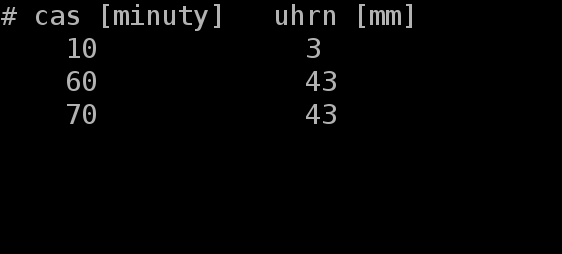
\includegraphics[width=0.5\textwidth]{./img/srazka.png}
  \caption{Ukázka srážkových dat. V intervalu 0 - 10 minut je úhrn 3 mm, v intervalu 10 - 60 minut je úhrn 40 mm a v intervalu 60 - 70 úhrn 0 mm}
  \label{fig:srazkovysoubor}
\end{figure}


\subsection{Časový krok modelu a celková doba simulace} \label{sec:vstupkrok}

Časový krok modelu označený \acs{dT} je hodnota v sekundách. Jako vstupní parametr se zadává maximální časový krok. Tento časový krok je rovněž počáteční časový krok. Časový krok je v průběhu výpočtu upravován podle Courantovy podmínky, tak aby bylo zachována numerická stabilita explicitního řešení. Velikost časového kroku závisí na rychlosti povrchového odtoku a na velikosti prostorového kroku (velikosti buňky DMT). Maximální časový krok záleží na požadovaném detailu výstupních dat zejména při dotoku srážkové epizody, kdy jsou již rychlosti proudění nižší a kde by v tom příkladě Courantova kritérium povolovalo příliš velký časový krok. Zvolené řešení změn časového kroku je detailněji popsáno v kapitole \ref{sec:cfl}. 

%Vzhledem k tomu, že rychlost odtoku v rýhám může být řádově vyšší než rychlost plošného odtoku je snaha řídit velikost časového kroku podle rychlosti plošného odtoku, kde Courantovo kritérium povoluje vyšší časový krok. Velikosti časového kroku zásadně ovlivňuje celkovou délku výpočtu. Pokud časový krok vyhovuje Courantovu kritériu v plošném odtoku, ale toku v rýhách již nikoli, začne se časový krok dělit pouze interně při výpočtu rýh. Tyto děje se probíhají při běhu programu a uživatel je nijak neovlivňuje, nicméně, je třeba si uvědomit, že při vytvoření rýhového odtoku a nutností dělit časový krok v těchto buňkách může se doba výpočtu jednoho časového kroku prodloužit. která udává velikost jednoho kroku výpočtu, v němž probíhá výpočet odtoku a další nedílné součásti programu. Zadaný časový krok se mění podle potřeb Courantova kritéria \ref{section:cfl}, nikdy však nemůže být vyšší než vstupní zadaná hodnota uživatelem. 

%Při zadávání počátečního časového kroku je možno zvolit hodnotu v rozmezí od 0.05 do 0.3 minuty. 
% Velikost časového kroku nejvíce ovlivňuje reálnou dobu běhu modelu. Čím nižší je časový krok, tím déle uživatel čeká na výsledky. 
%Stejně jako u všech ostatních číselných hodnot zadávaných do programu ArcGIS je potřeba myslet na to, že čísla s desetinnými místy musí být odděleny tečkou, nikoliv čárkou.
Délka běhu modelu je hodnota v minutách určující čas, do kterého se model po jednotlivých časových krocích dostane a skončí. Volba délky běhu modelu by měla dostatečně dlouhá, tak aby odtekla veškerá voda z řešeného území, především při zjišťován celkového objemu odtoku.
 


%\subsection{Povrchová retence} \label{sec:vstupretence}

%Povrchová retence je děj, při kterém se zachytává počáteční část srážky, která se dále neúčastní odtoku. V reálném prostředí si lze toto představit jako zachytávání srážkové vody v nerovnostech na povrchu. Pouze po naplnění těchto malých nerovností dochází k povrchovému odtoku. Hodnota závisí na hustotě půdy a její deformaci. Povrchová retence se zadává v mm. Pro veškerá testování byla povrchová retence zvolena 0.2 mm.

\subsection{Shapefile bodů pro generování hydrogramů} \label{sec:vstupbody}

Jedná  se o bodovou vrstvu. V těchto bodech se budou uživateli ukládat časové řady počítaných veličin. Tento volitelný vstupní parametr je podrobněji popsán ve výstupech \ref{sec:hydrogramy}.

\subsection{Výstupní adresář} \label{sec:vstupadresar}
Výstupní adresář je složka, do které se uloží veškeré výsledné rastry a výstupní textové soubory. Na začátku běhu programu se obsah tohoto adresář celý vymaže, proto se doporučuje vždy provést kontrolu. V žádném případě nenastavujete jako výstupní adresář pracovní plochu, či jiný adresář, kde byste mohli mít uložena důležitá data!

\subsection{Rýhový odtok} \label{sec:vstupryhovy}

Tento volitelný parametr po zaškrnutí umožní výpočet soustředěného odtoku. Soustředěný odtok je popsán v sekci \ref{sec:soustredenyodtok}.

\subsection{Vícesměrný odtok} \label{sec:vstupvicesmerny}

Parametr volby vícesměrného odtoku je volitelný. Více o tomto typu odtoku je v části \ref{subsection:MD}


\subsection{Hydrografická síť} \label{sec:vodnitoky}

Hydrografickou sítí jsou myšleny nejen vodní toky, ale i prvky dočasné hydrografické sítě jako jsou příkopy, průlehy, cesty s příkopy a pod. Výpočet v modelu probíhá po jednotlivých úsecích pomocí Manningovi rovnice pro výpočet průtoku. Prostorové umístění jednotlivých prvků je formou shapefile (\textbf{Vrstva toků - Stream feature}). Jednotlivé vektory reprezentují úsek se stejnými charakteristikami. Tvar úseku, drsnost, základní průtok jsou pak zadávány pomocí externí tabulky kde jsou uvedeny charakteristiky pro jednotlivé typy úseků (\textbf{Tabulka vodních toků - Stream table}). Pro propojení prostorové informace s charakteristikami úseků je třeba mít v atributové tabulce shodný kód jako ve vrstvě vodních toků (\textbf{Kód vodních toků - Steam table code}).






